\documentclass[12]{article}%12pt即为*四号字
\usepackage{ctex}%引入中文包
\usepackage{graphicx}%插入图片的包
\usepackage{geometry}%设置A4纸页边距的包
\usepackage{url}
\usepackage{stfloats}
\usepackage{float}
\usepackage{amssymb}
\geometry{left=3.18cm,right=3.18cm,top=2.54cm,bottom=2.54cm}%设置页边距
\linespread{1}%设置行间距



\begin{document}
\begin{center}
    \LARGE\songti\textbf{数值分析项目作业报告} \\%标题
    \large\kaishu\textbf{褚朱钇恒\qquad 3200104144}%一般是我的姓名
\end{center}
\section{运行说明}
    本项目需要调用\verb|jsoncpp|与\verb|eigen3|库,故请在运行此项目前安装好这两个包。

    在\verb|project|目录下使用\verb|make|命令即可编译整个项目并得到实验报告。

\section{程序设计思路}
所有实现样条计算的相关代码都在头文件\verb|spline.h|中,其中设计了一下几个类:
\subsection{Class Function}
其定义了\verb|()|,\verb|diff|,\verb|diff2|三个虚函数,分别用于函数求值,求导和求二阶导。

该基类有以下两个衍生类:
\begin{itemize}
    \item \verb|Class Polynomial| 用于存储一个多项式函数,形如$\Sigma Co_i(x-x_0)^i$
    \item \verb|Class B_spline_base| 用于存储一个$k$阶的B样条基函数,其控制点为$t$
\end{itemize}
\subsection{Class Interpolation}
定义了\verb|solve|,\verb|()|两个虚函数,分别用于插值系数计算和插值求值。
该基类有以下两个衍生类:
\begin{itemize}
    \item \verb|Class ppForm_interpolation| 用于使用多项式进行样条插值
    \item \verb|Class B_spline_base| 用于使用B样条基函数进行样条插值
\end{itemize}
以上两个衍生类可以在初始化时制定样条的阶数$order=1 or 3$,1对应线性样条,3对应三次样条($\mathbb{S}_3^2$);以及边界条件$condition=1 or 2 or 3$,m,1对应complete cubic spline,2对应cubic spline with specified second derivatives at its
end points,3对应natural cubic spline.

\section{作业题运行结果}
    \subsection{A}
        对不同的插值点数$N$,使用多项式样条拟合图像。结果如下:
        \begin{figure}[H]
            \centering
            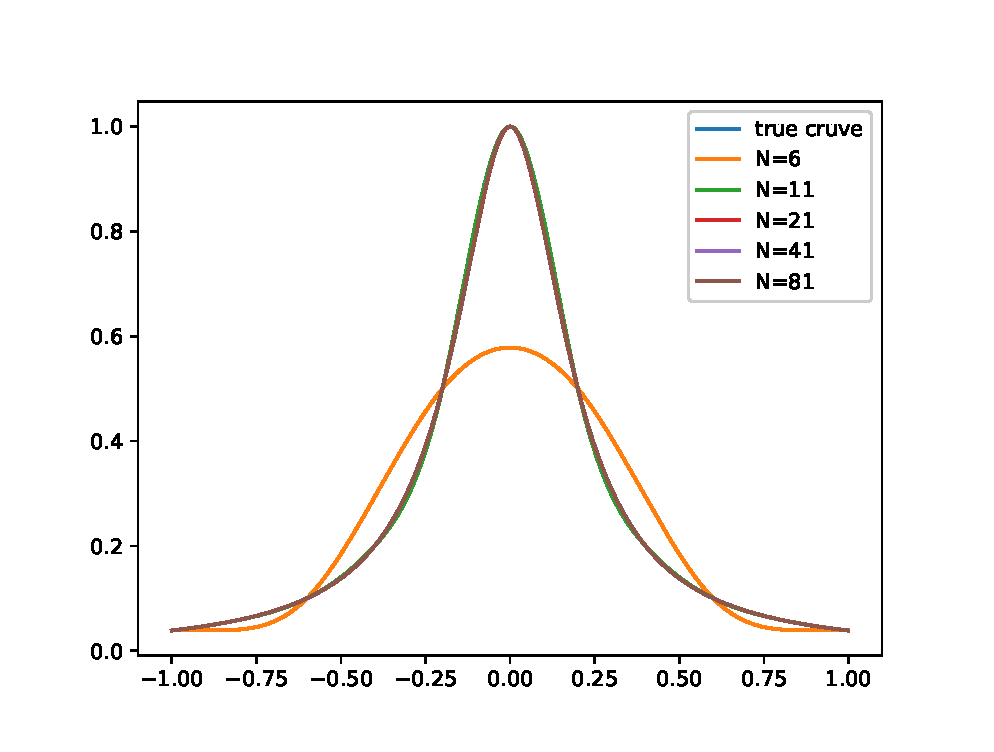
\includegraphics[width=0.7\textwidth]{../pic/A.eps}
            \caption{三次样条拟合图像}
        \end{figure}
        容易发现随着$N$的变大,拟合结果没有发生龙格现象,为了判断其究竟是否更加精准,此处做出其最大误差的自然对数和$N$的关系并作图。
        \begin{table}[]
            \begin{tabular}{|l|l|l|l|l|l|l|l|l|l|}
            \hline
            \multicolumn{1}{|r|}{N} & 6      & 11     & 21    & 41            & 81             & 161            & 321            & 641           & 801           \\ \hline
            err\_max                & 0.4217 & 0.0219 & 0.003 & $2.7*10^{-4}$ & $1.6*10^{-5}$ & $9.6*10^{-7}$ & $5.9*10^{-8}$ & $3.6*10^{-9}$ & $1.4*10^{-9}$ \\ \hline
            \end{tabular}
            \end{table}
        \begin{figure}[H]
            \centering
            \includegraphics[width=0.7\textwidth]{../pic/A2.eps}
            \caption{误差变化曲线}
        \end{figure}
        容易发现该样条的拟合精度随着$N$的变大而提升,其收敛阶至少大于3.
    
    \subsection{B}
        实现代码可见\verb|spline.h|
    \subsection{C}
        使用三次B样条和线性B样条分别拟合函数$f(x)=\frac{1}{1+x^2}$,结果如下图:
        \begin{figure}[H]
            \centering
            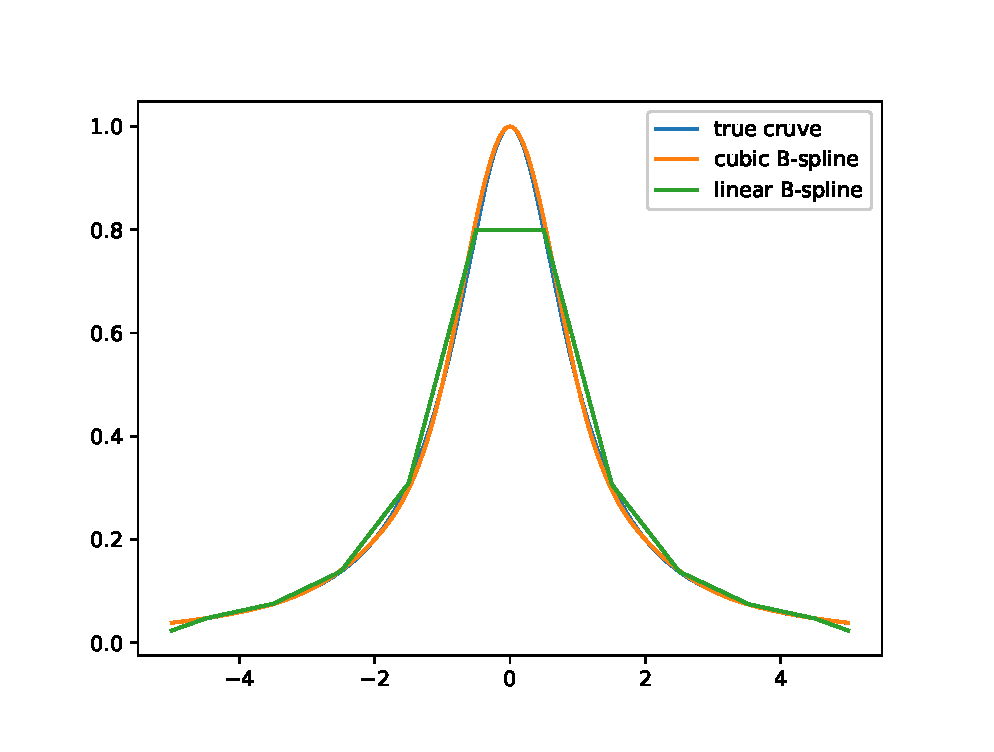
\includegraphics[width=0.7\textwidth]{../pic/C.eps}
            \caption{$f(x)=\frac{1}{1+x^2}$拟合结果}
        \end{figure}

        显然,三次样条的结果更精确。
    \subsection{D}
        问题C中的两个样条的误差如下图:
        \begin{figure}[H]
            \centering
            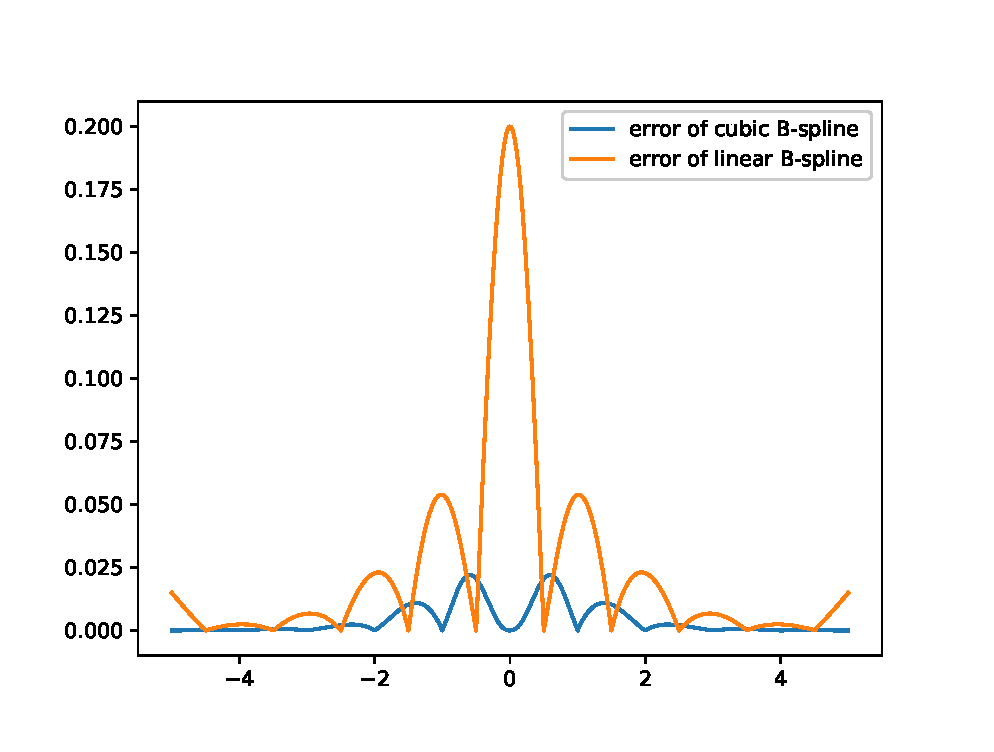
\includegraphics[width=0.7\textwidth]{../pic/C2.eps}
            \caption{误差变化曲线}
        \end{figure}

        可以发现在插值节点处的误差极小,接近机器精度,因为插值时我们给了这些位置的精确信息,故结果也很精确。

        此外从图像也可以看出,三次样条的误差更小。
    
    \subsection{E}
        将$(0,\pm\frac{2}{3}\sqrt{3}),\quad(\pm\sqrt{3},\frac{2}{3}\sqrt[4]{3})$设为特征点,使用三次B样条的拟合结果如下:
        \begin{figure}[H]
            \centering
            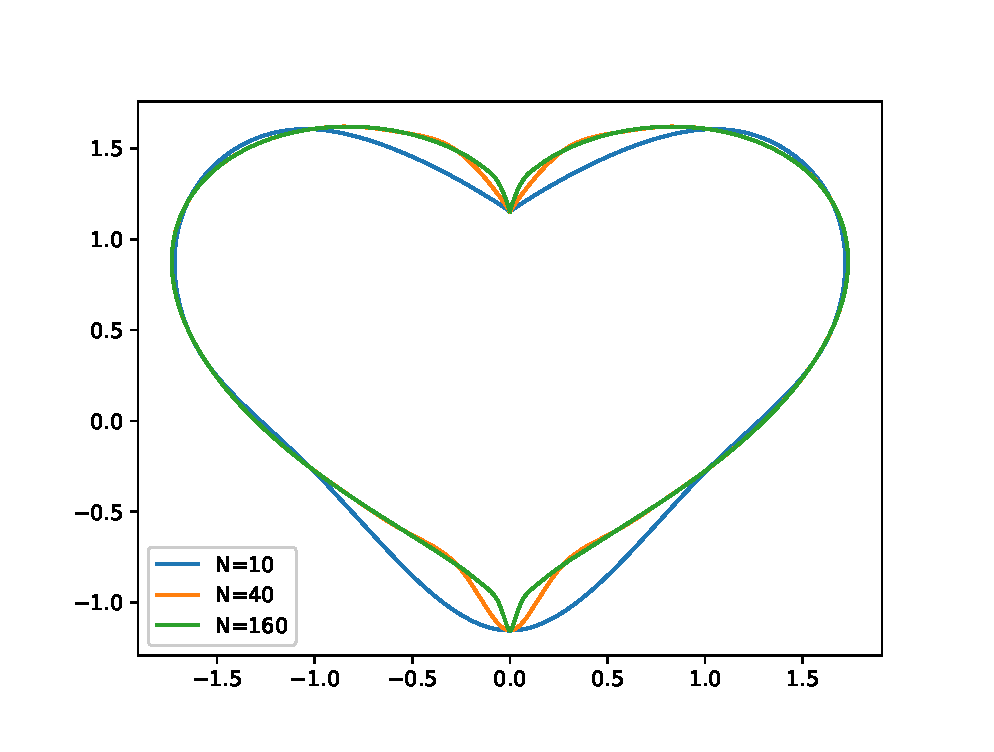
\includegraphics[width=0.7\textwidth]{../pic/E.eps}
            \caption{三次B样条心形拟合结果}
        \end{figure}

        从图像可以看出$N=40$时的拟合结果已经较为优秀。对于边界条件,natural cubic spline的边界条件最合适,因为离散的点值难以计算边界的导数,而规定其二阶导为0较为方便。

        使用线性样条的拟合结果如下:
        \begin{figure}[H]
            \centering
            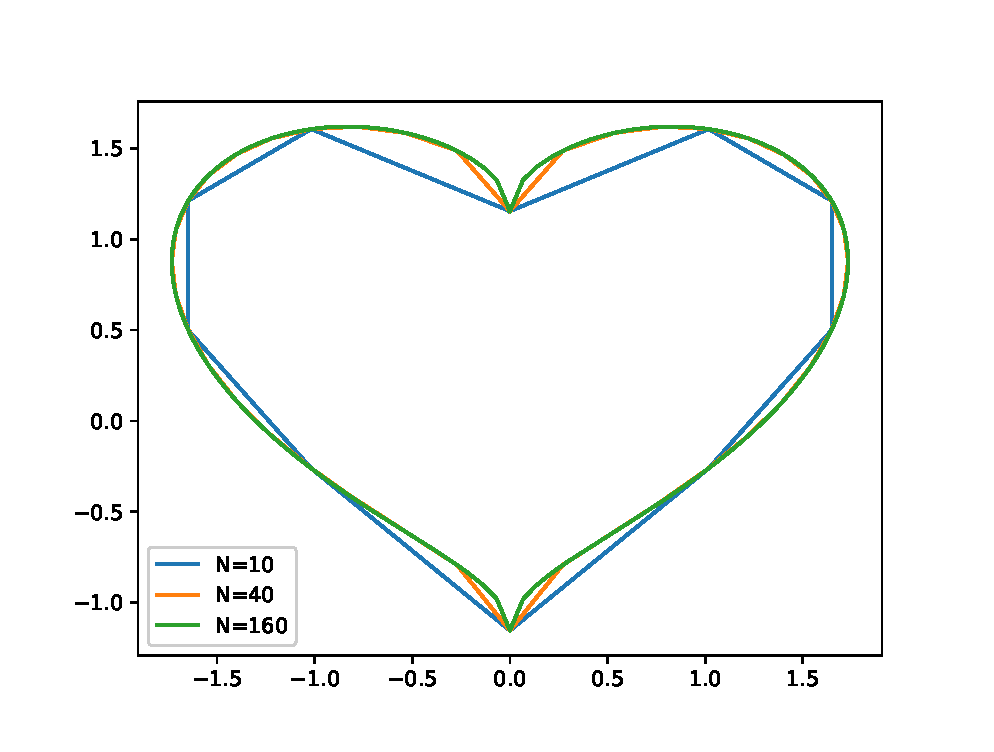
\includegraphics[width=0.7\textwidth]{../pic/E2.eps}
            \caption{线性样条心形拟合结果}
        \end{figure}

        从图像可以看出$N=40$时的拟合结果已经较为优秀。对于边界条件,线性样条不需要规定。

\end{document} 